% Options for packages loaded elsewhere
\PassOptionsToPackage{unicode}{hyperref}
\PassOptionsToPackage{hyphens}{url}
\PassOptionsToPackage{dvipsnames,svgnames,x11names}{xcolor}
%
\documentclass[
  letterpaper,
  DIV=11,
  numbers=noendperiod]{scrartcl}

\usepackage{amsmath,amssymb}
\usepackage{iftex}
\ifPDFTeX
  \usepackage[T1]{fontenc}
  \usepackage[utf8]{inputenc}
  \usepackage{textcomp} % provide euro and other symbols
\else % if luatex or xetex
  \usepackage{unicode-math}
  \defaultfontfeatures{Scale=MatchLowercase}
  \defaultfontfeatures[\rmfamily]{Ligatures=TeX,Scale=1}
\fi
\usepackage{lmodern}
\ifPDFTeX\else  
    % xetex/luatex font selection
\fi
% Use upquote if available, for straight quotes in verbatim environments
\IfFileExists{upquote.sty}{\usepackage{upquote}}{}
\IfFileExists{microtype.sty}{% use microtype if available
  \usepackage[]{microtype}
  \UseMicrotypeSet[protrusion]{basicmath} % disable protrusion for tt fonts
}{}
\makeatletter
\@ifundefined{KOMAClassName}{% if non-KOMA class
  \IfFileExists{parskip.sty}{%
    \usepackage{parskip}
  }{% else
    \setlength{\parindent}{0pt}
    \setlength{\parskip}{6pt plus 2pt minus 1pt}}
}{% if KOMA class
  \KOMAoptions{parskip=half}}
\makeatother
\usepackage{xcolor}
\setlength{\emergencystretch}{3em} % prevent overfull lines
\setcounter{secnumdepth}{-\maxdimen} % remove section numbering
% Make \paragraph and \subparagraph free-standing
\ifx\paragraph\undefined\else
  \let\oldparagraph\paragraph
  \renewcommand{\paragraph}[1]{\oldparagraph{#1}\mbox{}}
\fi
\ifx\subparagraph\undefined\else
  \let\oldsubparagraph\subparagraph
  \renewcommand{\subparagraph}[1]{\oldsubparagraph{#1}\mbox{}}
\fi


\providecommand{\tightlist}{%
  \setlength{\itemsep}{0pt}\setlength{\parskip}{0pt}}\usepackage{longtable,booktabs,array}
\usepackage{calc} % for calculating minipage widths
% Correct order of tables after \paragraph or \subparagraph
\usepackage{etoolbox}
\makeatletter
\patchcmd\longtable{\par}{\if@noskipsec\mbox{}\fi\par}{}{}
\makeatother
% Allow footnotes in longtable head/foot
\IfFileExists{footnotehyper.sty}{\usepackage{footnotehyper}}{\usepackage{footnote}}
\makesavenoteenv{longtable}
\usepackage{graphicx}
\makeatletter
\def\maxwidth{\ifdim\Gin@nat@width>\linewidth\linewidth\else\Gin@nat@width\fi}
\def\maxheight{\ifdim\Gin@nat@height>\textheight\textheight\else\Gin@nat@height\fi}
\makeatother
% Scale images if necessary, so that they will not overflow the page
% margins by default, and it is still possible to overwrite the defaults
% using explicit options in \includegraphics[width, height, ...]{}
\setkeys{Gin}{width=\maxwidth,height=\maxheight,keepaspectratio}
% Set default figure placement to htbp
\makeatletter
\def\fps@figure{htbp}
\makeatother

\KOMAoption{captions}{tableheading}
\makeatletter
\@ifpackageloaded{caption}{}{\usepackage{caption}}
\AtBeginDocument{%
\ifdefined\contentsname
  \renewcommand*\contentsname{Table of contents}
\else
  \newcommand\contentsname{Table of contents}
\fi
\ifdefined\listfigurename
  \renewcommand*\listfigurename{List of Figures}
\else
  \newcommand\listfigurename{List of Figures}
\fi
\ifdefined\listtablename
  \renewcommand*\listtablename{List of Tables}
\else
  \newcommand\listtablename{List of Tables}
\fi
\ifdefined\figurename
  \renewcommand*\figurename{Figure}
\else
  \newcommand\figurename{Figure}
\fi
\ifdefined\tablename
  \renewcommand*\tablename{Table}
\else
  \newcommand\tablename{Table}
\fi
}
\@ifpackageloaded{float}{}{\usepackage{float}}
\floatstyle{ruled}
\@ifundefined{c@chapter}{\newfloat{codelisting}{h}{lop}}{\newfloat{codelisting}{h}{lop}[chapter]}
\floatname{codelisting}{Listing}
\newcommand*\listoflistings{\listof{codelisting}{List of Listings}}
\makeatother
\makeatletter
\makeatother
\makeatletter
\@ifpackageloaded{caption}{}{\usepackage{caption}}
\@ifpackageloaded{subcaption}{}{\usepackage{subcaption}}
\makeatother
\ifLuaTeX
  \usepackage{selnolig}  % disable illegal ligatures
\fi
\usepackage{bookmark}

\IfFileExists{xurl.sty}{\usepackage{xurl}}{} % add URL line breaks if available
\urlstyle{same} % disable monospaced font for URLs
\hypersetup{
  pdftitle={Renewable NEM 2 - with transmission},
  pdfauthor={David Leitch and Paul Bandarian},
  colorlinks=true,
  linkcolor={blue},
  filecolor={Maroon},
  citecolor={Blue},
  urlcolor={Blue},
  pdfcreator={LaTeX via pandoc}}

\title{Renewable NEM 2 - with transmission}
\author{David Leitch and Paul Bandarian}
\date{2024-03-28}

\begin{document}
\maketitle

\section{Renewable NEM from scratch part 2 - includes
transmission}\label{renewable-nem-from-scratch-part-2---includes-transmission}

As discussed in our Part 1 of our renewable NEM, ITK built a renewable
NEM from scratch, aimed at meeting NEM-wide CY2025 demand. We focussed
on generating a VRE portfolio with the highest Sharpe ratio, that is,
the portfolio where average output could not be increased without also
increasing variability. That study took no account of transmission.

In Part 2 below, we include an estimate of transmission but still
require the portfolio to have VRE meeting a series of targeted
``Sharpe'' ratios; the ratio becoming a constraint, while the optimiser
minimises cost. AEMO-modelled demand for CY2025 must be met in every
half-hour period by the modelled VRE portfolio in combination with a
fixed quantity of hydro (equal to historic NEM output), storage (pumped
hydro, or more likely batteries) and variable quantity of gas. As hydro
and storage output were fixed throughout the analysis, the quantity of
gas power and gas generation are outputs of the model. A map of ITK's
preferred VRE portfolio -- with the constraint Sharpe ratio ≥ 4 -- is
shown in Figure 1 below.

\begin{figure}[H]

{\centering 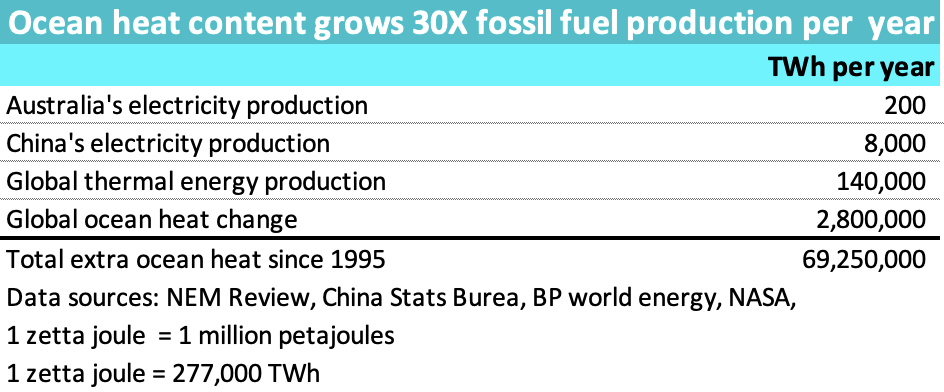
\includegraphics[width=3.49583in,height=5.46875in]{./media/media/image1.png}

}

\caption{Preferred portfolio. Source:ITK}

\end{figure}%

Figure 1: ITK Preferred VRE Portfolio Map

We use the portfolios generated to estimate the resulting electricity
price that would provide a net present value (NPV) of zero in each case.
Based on our (no doubt optimistic) cost assumptions, these prices turn
out to be in the \$60-\$70 / MWh range, similar to that of consultants
who looked at the NSW, Queensland and Victorian grid decarbonisation
plans. If nothing else, this demonstrates that spending \$200bn doesn't
result in a dramatic increase in electricity prices, quite the reverse.
Eliminating most fuel and other variable costs leads to a stable and
predictable price that is globally competitive. Our cost estimate does
not include rooftop solar; it is taken as a ``free good''. The authors
learned a lot from this exercise, and we are grateful to AEMO for the
data that makes such studies possible.

\subsection{Key Findings}\label{key-findings}

Based on the results from these desktop studies and subject to the
numerous limitations discussed herein:

\textbf{Targeting improved system reliability and reduced emissions
drives} \textbf{the model towards greater reliance on wind, particularly
situated at the} \textbf{fringes of the grid. This approach necessitates
a more interconnected} \textbf{NEM and therefore increased initial
investment in transmission networks} \textbf{but reduced firming costs
in the long run.}

The lowest cost solutions feature greater solar capacity, located closer
to demand centres but extra firming gas to deal with resulting
volatility. Figure 2 and Table 1 illustrate the two extremes, namely
minimum cost over a short amortisation period and maximum system
stability.

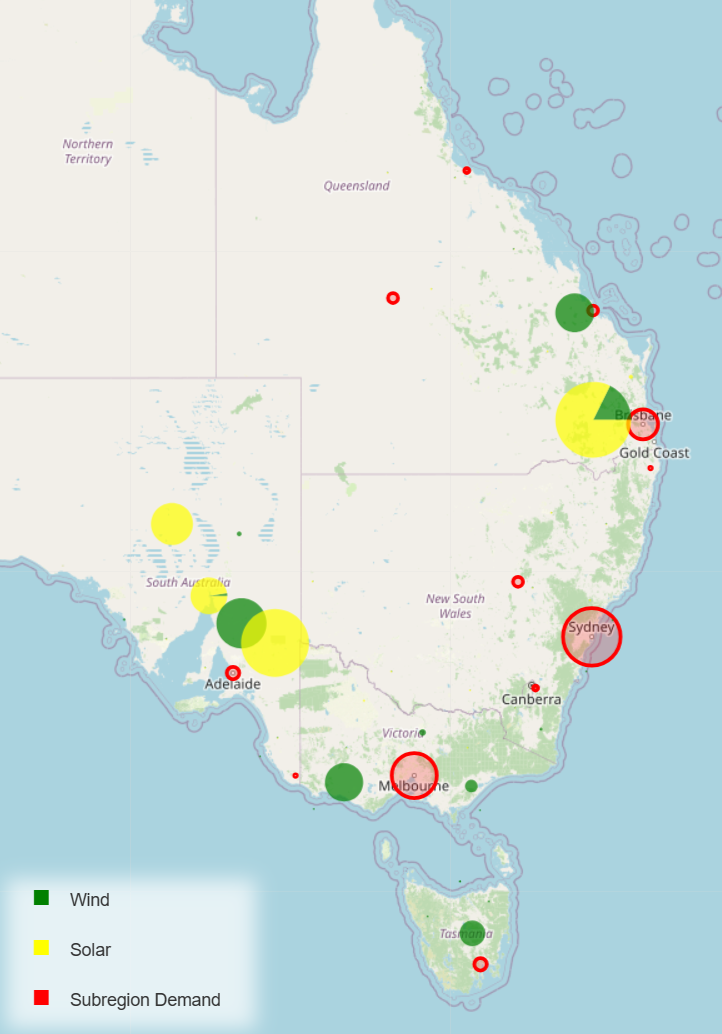
\includegraphics[width=3.63472in,height=5.20556in]{./media/media/image3.png}
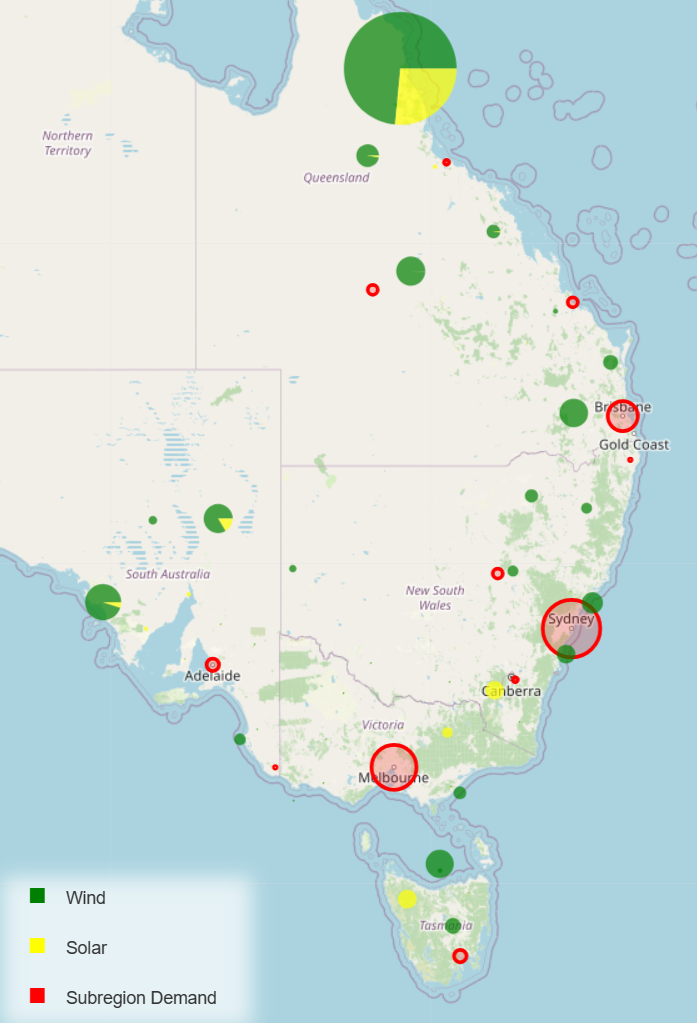
\includegraphics[width=3.55in,height=5.20972in]{./media/media/image5.png}

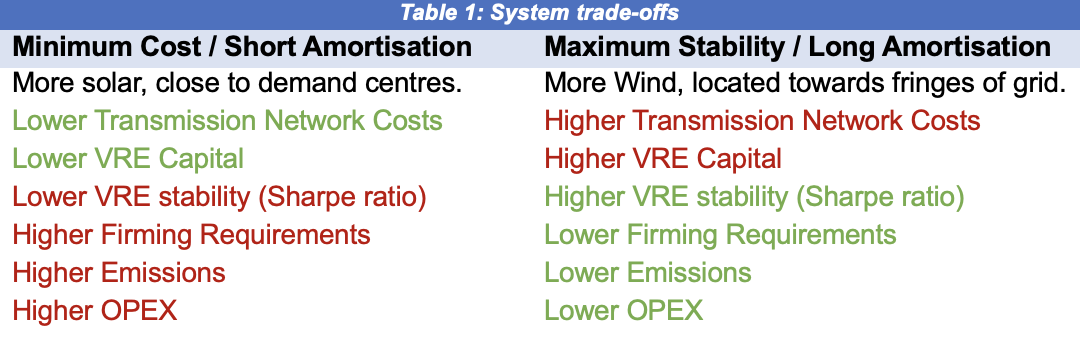
\includegraphics[width=6.26806in,height=1.8in]{./media/media/image7.png}

Amortising the system's capital costs over longer periods yields similar
results to increasing system reliability and reducing emissions. Namely,
the compounding cost of fuel to supply firming gas plants over a longer
period acts to disincentivise solar, driving greater reliance on wind
energy especially at the fringes of the grid and, again, a more
interconnected NEM. Figure 3 shows the Capital + 25-Year OPEX costs of
systems modelled to minimize cost over 10-, 15-, 20-, and 25-year
periods respectively.

\begin{figure}[H]

{\centering 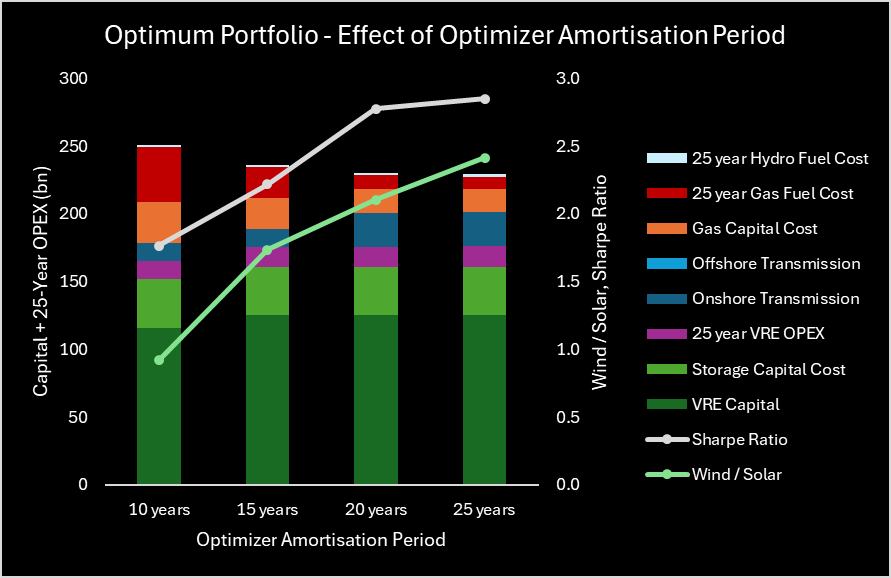
\includegraphics[width=5.94028in,height=3.85347in]{./media/media/image8.png}

}

\caption[25-Year Cost Breakdown for Portfolio Optimized at 10-, 15-, 20-
\& 25-Years Amortization]{25-Year Cost Breakdown for Portfolio Optimized at 10-, 15-, 20-
\& 25-Years Amortization\footnotemark{}}

\end{figure}%
\footnotetext{The optimiser is programmed to
  generate the lowest cost portfolio over 10, 15, 20 and 25 years
  respectively. The cost breakdown indicated is the 25-year total system
  cost for each of these portfolios.}

With slightly higher upfront investment -- compared to the lowest cost
solution -- we can significantly reduce carbon emissions and improve VRE
portfolio stability by building a highly-interconnected system more
heavily weighted towards quality wind assets at the fringes of the grid.
To achieve this practically, ITK's preferred VRE portfolio minimizes
total system cost over 25 years subject to exceeding a minimum system
reliability requirement (Sharpe ratio ≥ 4). See Figure 4 which shows
cost breakdown for three key scenarios.

\begin{figure}[H]

{\centering \includegraphics[width=5.57361in,height=3.77361in]{./media/media/image9.png}

}

\caption{Cost Breakdown and Mt CO\textsubscript{2}-e for: Min Cost, ITK
Preferred, and Sharpe-Optimized Portfolios}

\end{figure}%

In virtually all simulations and sensitivities, QLD ends up as a
significant supplier of VRE and were it not for the higher costs of
underwater DC transmission, TAS would also be favoured as a large
exporter of wind. More wind in QLD -- particularly in the Northern half
of QLD -- and more QLD/NSW interconnect capacity will be ``low regrets''
options in building out the low carbon NEM.

\begin{figure}[H]

{\centering 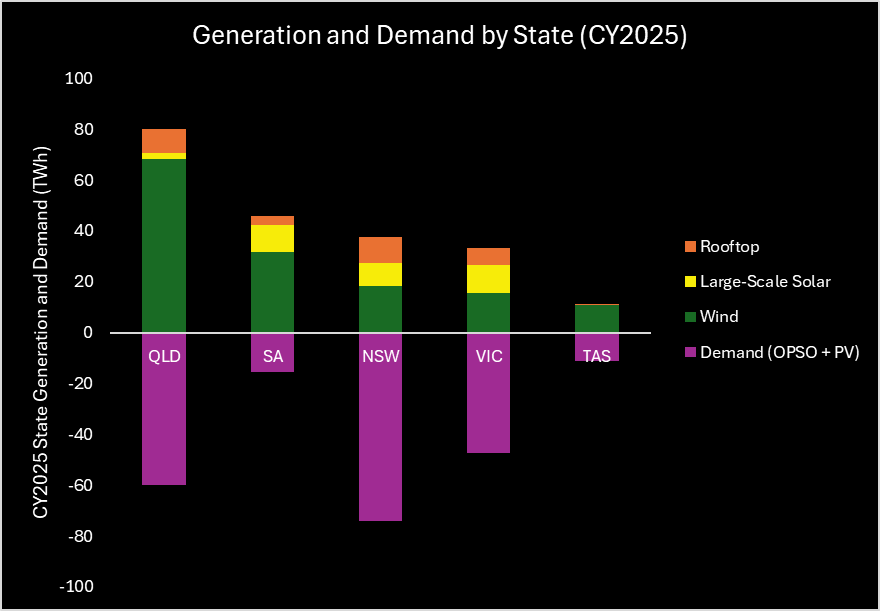
\includegraphics[width=5.86736in,height=4.07361in]{./media/media/image10.png}

}

\caption[ITK Preferred Portfolio Generation and Demand per State.]{ITK Preferred Portfolio Generation and Demand\footnotemark{} per State.}

\end{figure}%
\footnotetext{Demand
  values shown below the x-axis (negative)}

\subsection{Method}\label{method}

Starting with a fresh sheet of paper, we build a wind and solar
portfolio from AEMO's renewable energy zones (REZ's) -- as detailed in
the 2024 Draft Integrated System Plan (ISP) -- add in existing behind
the meter, and firm it with batteries, hydro, and gas to meet NEM-wide
operational demand in every half-hour period for the calendar year 2025.
We build multiple such systems using an optimization algorithm, each
time varying the set of constraints/incentives given to the optimizer.
The system constraints in each scenario are a combination of:

\begin{enumerate}
\def\labelenumi{\arabic{enumi}.}
\item
  Volatility minimization -- The \emph{Sharpe ratio} of a portfolio is
  inversely proportional to its variability. Practically, we sought to
  maximise the stability of the VRE portfolio by increasing its Sharpe
  ratio.
\item
  Cost Minimization -- Costs included:

  \begin{enumerate}
  \def\labelenumii{\alph{enumii}.}
  \item
    VRE Portfolio capital cost and fixed OPEX.
  \item
    Transmission Network capital cost.
  \item
    Storage capital cost.
  \item
    Firming Gas capital cost and running fuel cost.
  \item
    Hydro OPEX.
  \end{enumerate}
\item
  TAS Generation limit -- When stated, we assume that Tasmanian
  generation surplus to state demand must be transmitted to Victoria,
  therefore incurs DC transmission costs.
\item
  REZ generation limits -- Capacity of wind and solar for each REZ are
  set to the ``Renewable Potential (MW)'' values stated in AEMO's 2024
  Draft ISP.
\item
  VRE Portfolio generation -- represented as the ratio \emph{VRE
  Portfolio Gen / NEM CY25 Demand}. Sensitivity analysis shows that
  \textasciitilde100\% - 110\% of NEM CY25 demand is ideal.
\item
  Years' OPEX included in total system cost.
\end{enumerate}

Battery power and storage are fixed at \textbf{\emph{15 GW}} and
\textbf{\emph{4 hours}}. Hydro power and capacity are fixed at
\textbf{\emph{7.5 GW}} and \textbf{\emph{14 TWh}}. These values could be
optimized in future simulations, as we know that for any given VRE
portfolio, more battery/hydro means less gas and vice versa.

\subsection{Firming}\label{firming}

A VRE portfolio with annual output equal to or greater than demand in
the NEM inevitably requires ``firming'' supplied by some combination of
storage, hydro and gas. In designing such a system there are various
trade-offs between transmission and firming costs. Systems built to
minimize the total firming requirement will end up with more wind, much
of which will be located around the perimeter of the grid, and therefore
result in greater transmission requirements. Once transmission costs are
allowed for, a lower overall cost solution is to have more solar located
closer to demand, and to handle the resulting volatility with extra
firming using gas.

A feature of a high VRE grid is strong seasonality. Output from solar is
lower in winter and wind is also seasonal. When only batteries or pumped
hydro are used to deal with wind and solar supply shortfalls our work
shows that, for any ``reasonable'' quantity of storage, it is often
empty. This is particularly the case in winter. Our analysis shows that
using gas earlier in the merit order during winter resulted in lower
requirement for storage capacity while retaining ``low'' gas
consumption. By contrast, using storage early in the supply sequence
during spring and summer -- when VRE output tends to exceed demand --
minimises the use of gas.

We note that once again QLD output helps with seasonality droughts, as
QLD wind tends to be better in Winter and less in Summer.

\subsection{Sharpe Ratio}\label{sharpe-ratio}

The Sharpe ratio of a portfolio is inversely proportional to its
variability. Average output of the Sharpe ratio-maximised portfolio
cannot be increased without incurring more volatility. Practically, we
first maximised the stability of the VRE portfolio by increasing its
Sharpe ratio. This showed that the highest Sharpe ratio portfolio was
dominated by Qld and Tasmania onshore wind, but also included about 19\%
solar and a small amount of offshore wind. A major limitation of this
analysis being the omission of transmission costs.

Subsequently we estimate the cost\footnote{In this note costs are not
  intended to be indicative of actual costs but rather goals set in the
  optimisation function} of the system (capital costs, transmission
network costs and OPEX) and generate several cost-minimised portfolios,
gradually introducing minimum Sharpe ratio constraints. Increasing the
minimum Sharpe ratio requirement of the cost-optimizer incentivises
widening the geographical distribution of power generation, i.e., more
generation near the fringes of the grid. This is intuitive: generally,
the greater the distance between two REZ's the less correlation there is
between the weather conditions at the two locations, particularly for
wind. This effect is clearly observed in the correlation matrices of the
wind and solar capacity factors (Figure 6 and Figure 7).

\begin{figure}[H]

{\centering \includegraphics[width=6.17706in,height=6in]{./media/media/image11.jpeg}

}

\caption{REZ Solar Capacity Factor Correlation Matrix - Ordered by
Latitude}

\end{figure}%%
\begin{figure}[H]

{\centering 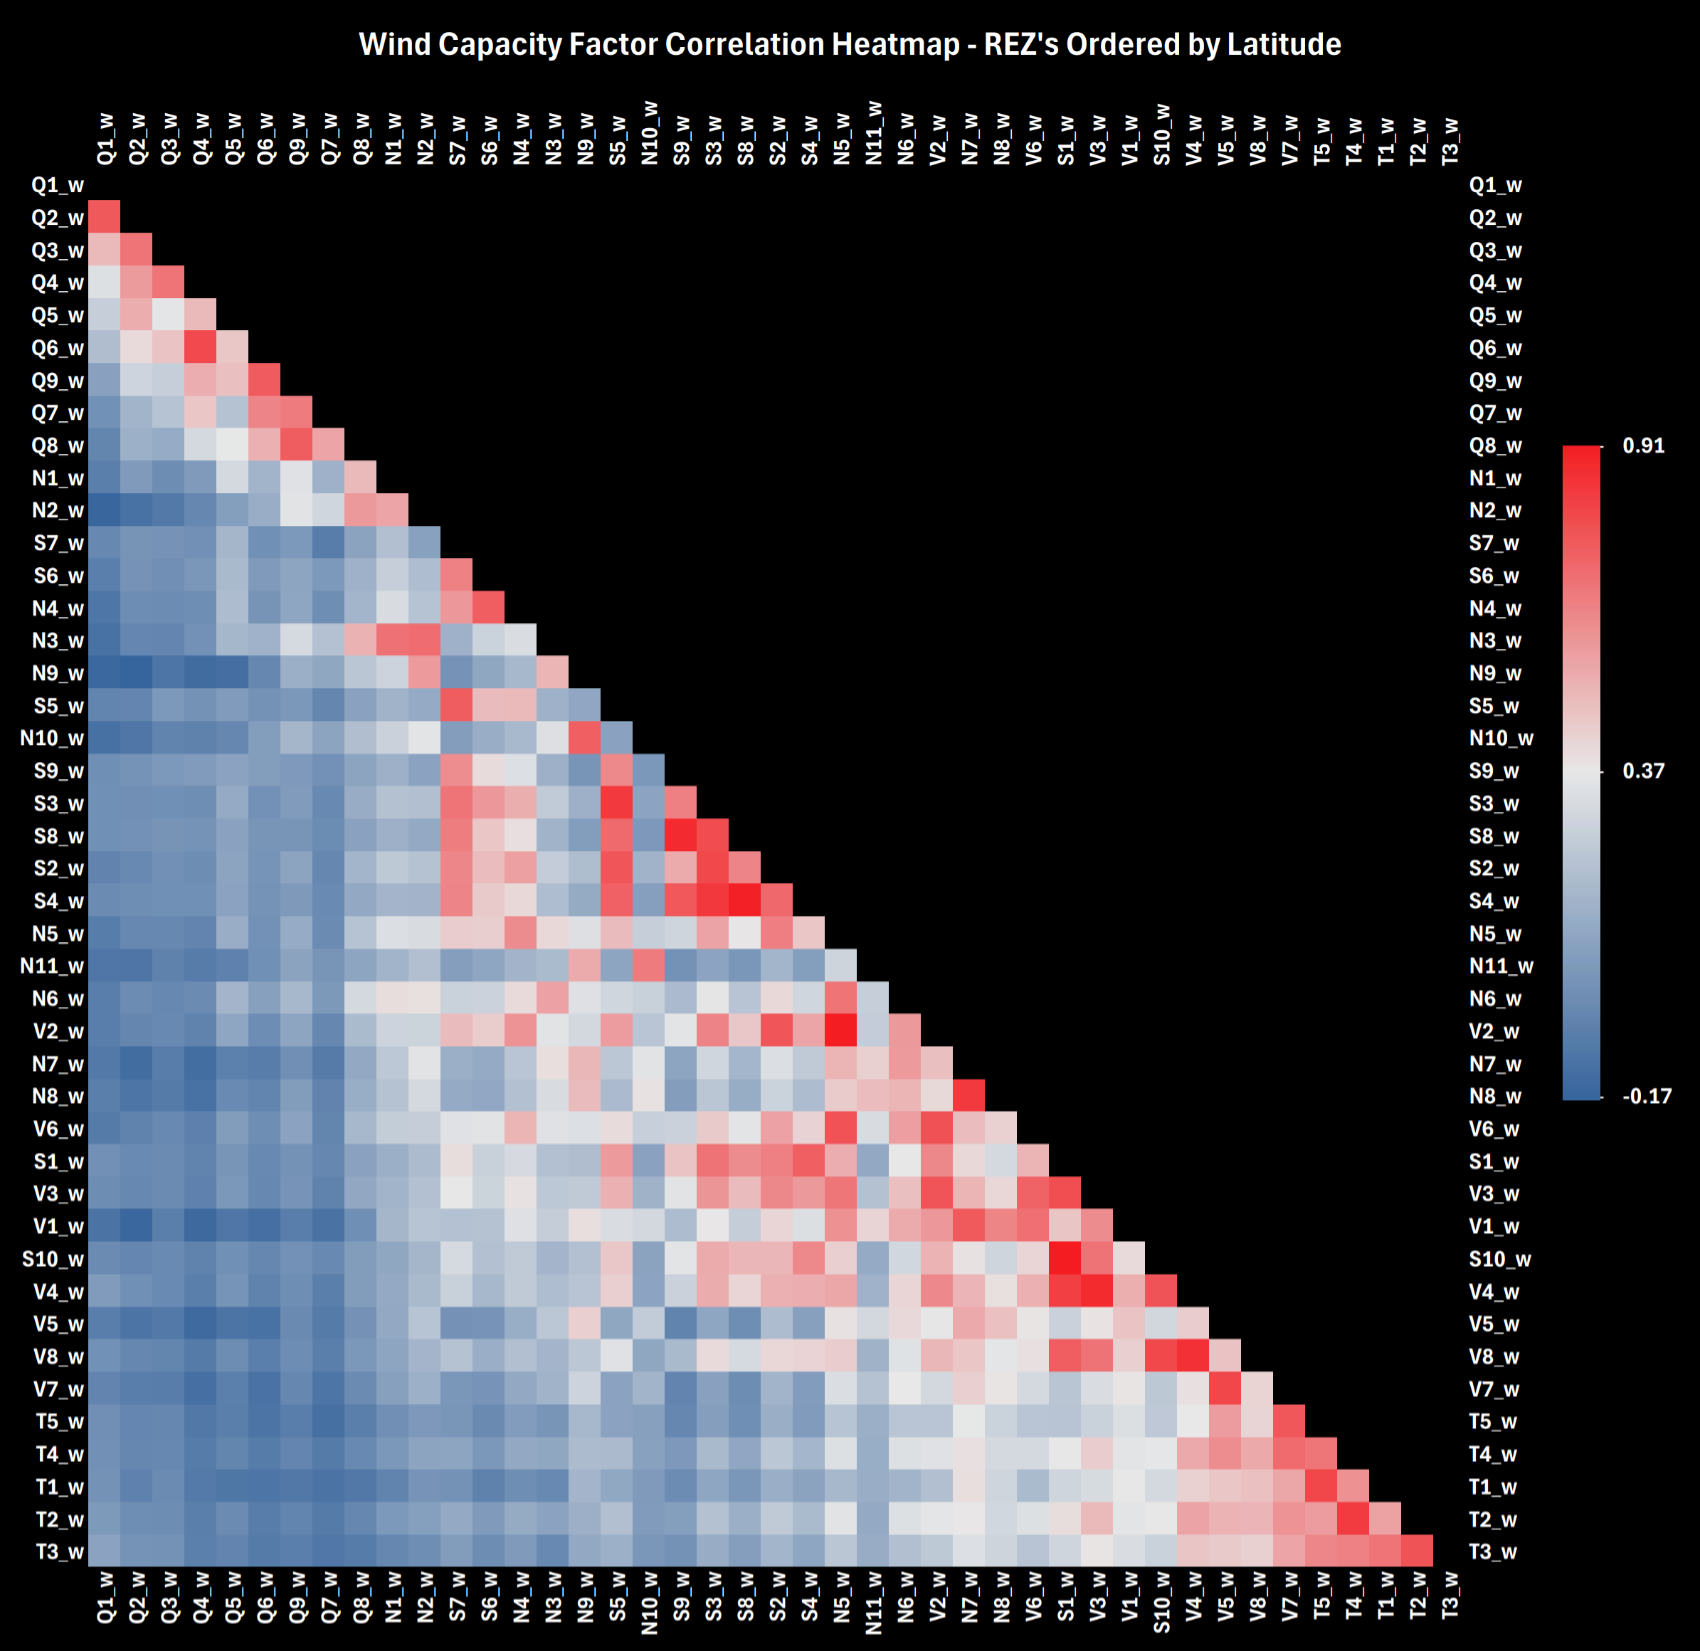
\includegraphics[width=6.88333in,height=6.68471in]{./media/media/image12.png}

}

\caption{REZ Wind Capacity Factor Correlation Matrix - Ordered by
Latitude}

\end{figure}%

In a Sharpe-optimised system, there is a lot of incentive to allocate
weight to REZ's in Northern Queensland (farthest North), Central South
Australia (farthest West) and Tasmania (farthest South) as this achieves
the widest possible geographic spread of generation. We see this
assertion supported in Figure 2.

Increasing the Sharpe ratio also incentivises wind -- particularly Tas
and Qld wind -- over solar, again intuitively, because:

\begin{enumerate}
\def\labelenumi{(\alph{enumi})}
\item
  the power generation of a higher-Sharpe-ratio portfolio would drop
  less drastically overnight.
\item
  Solar capacity factors from separate REZ's have a much stronger
  correlation with each other than wind capacity factors. Increasing
  wind in the portfolio therefore has a greater upwards influence on
  Sharpe ratio than solar. See Table 2. The Sharpe ratio of an evenly
  weighted solar-only portfolio is about a third of the Sharpe ratio of
  an evenly weighted wind-only portfolio.
\end{enumerate}

Table 2: Sharpe Ratio for Solar and Wind Only\\
Portfolios

\textbf{Portfolio Sharpe Ratio}

Solar Only (Evenly Weighted) 0.83

Wind Only (Evenly Weighted) 2.52

\subsection{Impact of constraining Sharpe ratio
higher}\label{impact-of-constraining-sharpe-ratio-higher}

As we increase the minimum acceptable Sharpe ratio (model constraint) in
our cost minimisation model we observe:

\begin{enumerate}
\def\labelenumi{\arabic{enumi}.}
\item
  More generation at the fringes of the grid, therefore higher onshore
  transmission cost.
\item
  VRE portfolio weight more heavily allocated to wind.
\item
  Lower firming requirements -- and therefore lower gas capital and fuel
  costs -- as the more stable portfolio with higher wind meets NEM
  demand in a greater portion of half-hour periods. This has an
  exaggerated effect on the system balance through peak demand, and
  overnight, as solar trails off.
\end{enumerate}

Figure 8 illustrates the effect of increasing the Sharpe ratio on the
average day power supply by source (i.e., more VRE, less firming).

\begin{figure}[H]

{\centering \includegraphics[width=7.26806in,height=4.79236in]{./media/media/image13.gif}

}

\caption{Average Day Supply by Source at Different Sharpe Ratios}

\end{figure}%

\subsection{VRE portfolio scale impact on
cost}\label{vre-portfolio-scale-impact-on-cost}

As VRE Portfolio capacity relative to NEM demand (``VRE Scale'' hereon)
increases, system capital cost increases but firming capacity
requirements decrease. To minimise long term costs, VRE portfolio
generation should be set to 100-110\% of CY2025 demand. See Figure 9,
which models the costs of ITK's preferred portfolio at various values of
VRE Scale. The optimal setpoint for this ratio achieves the best
trade-off between VRE capital costs and gas fuel costs. Although
slightly more costly, 110\% VRE Scale was preferred, because it had
substantially lower gas requirements than 100\%.

\begin{figure}[H]

{\centering 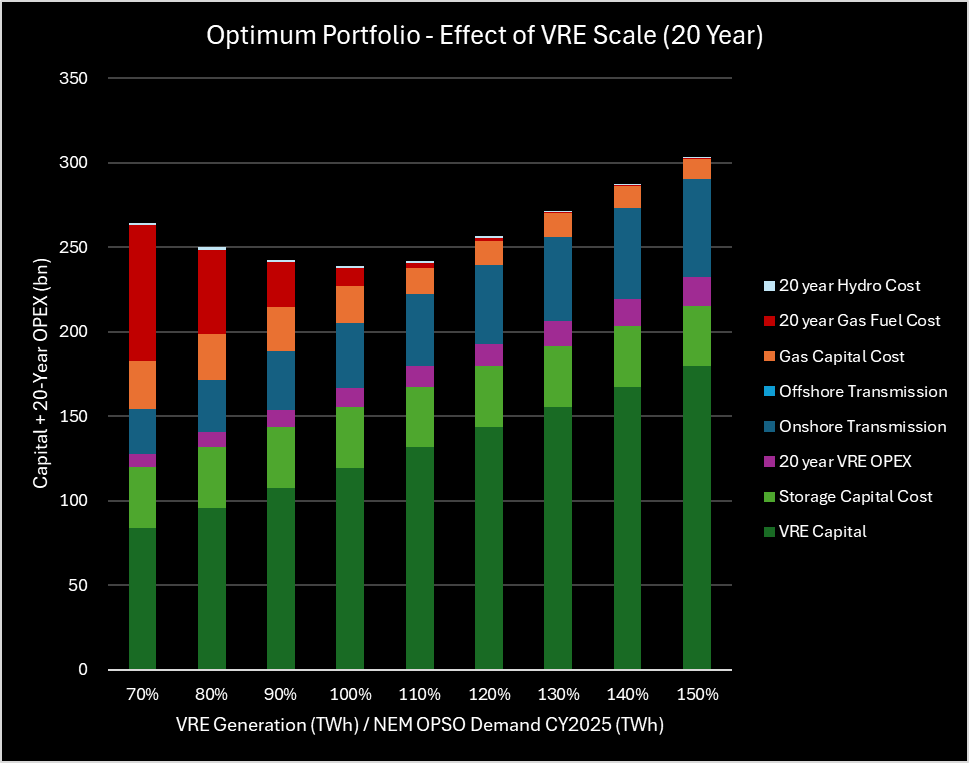
\includegraphics[width=6.46042in,height=5.08681in]{./media/media/image14.png}

}

\caption{Effect of "VRE Scale" on System Cost and OPEX}

\end{figure}%

\subsection{Impact of solar as share of
VRE}\label{impact-of-solar-as-share-of-vre}

A similar sensitivity analysis was conducted on the Wind / Solar ratio,
by varying the relative amount of each within the portfolio (retaining
REZ ratios within each generation type). The optimum mix sits at around
18.5\% Solar (using Draft ISP 2024 data). The greater the solar, the
lower the capital cost, but this comes at the expense of significantly
higher firming requirements, and therefore higher long-term cost.

\begin{figure}[H]

{\centering \includegraphics[width=6.12083in,height=4.44722in]{./media/media/image15.png}

}

\caption{Effect of VRE Portfolio \% Solar on System Cost and OPEX}

\end{figure}%

\subsection{ITK preferred portfolio}\label{itk-preferred-portfolio}

ITK prefers a slightly more expensive system (than the absolute minimum
cost) with greater transmission requirements but significantly lower
reliance on gas. This portfolio minimizes the 25-year total cost of the
system with the following additional requirements:

\begin{enumerate}
\def\labelenumi{\arabic{enumi}.}
\item
  a Sharpe ratio ≥ 4.0 (set as a constraint in the optimisation model)
\item
  VRE scaled to generate 110\% of NEM total demand in CY2025, and
\item
  Tas generation surplus to state demand must be transmitted to
  Victoria, therefore incurs offshore transmission costs. Given the high
  cost of DC transmission, this constraint renders Tas generation
  surplus to state demand nonviable.
\end{enumerate}

\begin{figure}[H]

{\centering 
\includegraphics[width=3.88056in,height=3.54028in]{./media/media/image16.png}

}

\caption{ITK-Preferred VRE Portfolio Supply by Source}

\end{figure}%

ITK's preferred portfolio consists of:

\begin{enumerate}
\def\labelenumi{\alph{enumi}.}
\item
  \textbf{\emph{58 GW}} of VRE supplying \textbf{\emph{160 TWh}} in
  CY2025.
\item
  \textbf{\emph{15 GW}} / \textbf{\emph{4h}} of BESS supplying
  \textbf{\emph{3.8 TWh}} in CY2025.
\item
  \textbf{\emph{13 GW}} of firming gas supplying \textbf{\emph{1.5 TWh}}
  in CY2025.
\item
  \textbf{\emph{7.5}} \textbf{\emph{GW}} / \textbf{\emph{14}}
  \textbf{\emph{TWh}} of Hydro supplying \textbf{\emph{12 TWh}} in
  CY2025.
\end{enumerate}

\subsection{Costs}\label{costs}

In this note, costs are not intended to be indicative of actual costs
but rather are goals set in the optimisation function. Specifically, the
optimiser takes no account of existing assets other than hydro. No
account is taken of existing gas, existing wind and solar or existing
transmission.

Equally because the VRE and storage are built on an ``overnight'' basis,
no allowance is made for learning rate impacts which are expected to
drive down the costs of solar and batteries, particularly over the next
decade. ITK's personal expectation is that once we get into the
transmission building phase of the transition that some improvement in
the cost outlook for this component can be achieved.

That said the unit costs and weights of three systems that we built are
shown in Table 3:

\begin{enumerate}
\def\labelenumi{\arabic{enumi}.}
\item
  \textbf{Lowest cost portfolio}, 25-year total cost minimised, Tas
  generation constrained\footnote{Tas generation above state demand
    incurs offshore transmission costs, as it must be transmitted to
    Victoria.}
\item
  \textbf{ITK's preferred portfolio}, 25-year total cost minimised, Tas
  generation constrained, VRE portfolio Sharpe Ratio ≥ 4.
\item
  \textbf{Sharpe-optimised portfolio}. No cost constraint, Sharpe ratio
  maximised.
\end{enumerate}

\begin{figure}[H]

{\centering 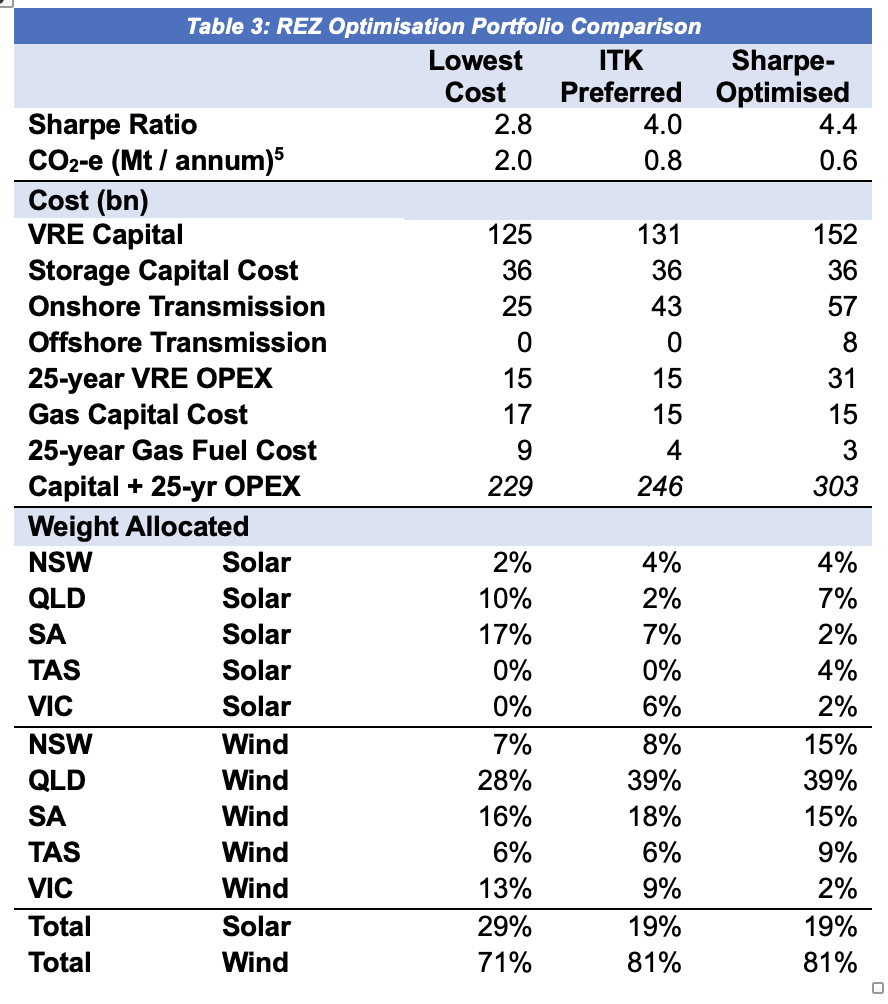
\includegraphics[width=6in,height=4.8in]{./media/media/image17.png}

}

\caption{A table with numbers and percentages Description automatically
generated}

\end{figure}%

Table 4 details our cost input assumptions.

\begin{figure}[H]

{\centering 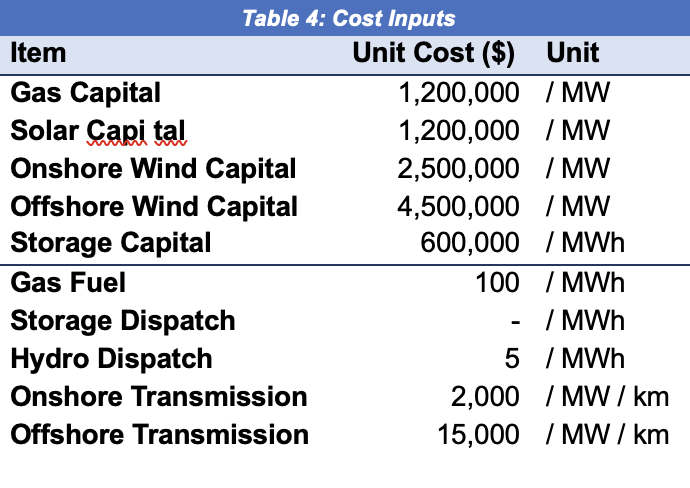
\includegraphics[width=4.79167in,height=3.38889in]{./media/media/image18.png}

}

\caption{Input cost assumptions. Source:ITK}

\end{figure}%

To find the price of electricity required to justify the investment, we
ran an NPV analysis and set the price at a level which ensures an
internal rate of return (IRR) equal to the weighted average cost of
capital (WACC). This required all assets, both new and existing, to earn
a return on capital and recover all OPEX.

A shortcut to this process is to take our capital costs per Table 4, add
in a cost of \$3m / MW for 7500 MW of existing hydro, and also allow
\$12 / MWh for wind and \$5 / MWh for solar OPEX, solely for this
specific levelized cost objective. This analysis yielded the following
required electricity prices:

\begin{figure}[H]

{\centering \includegraphics[width=4.875in,height=1.25in]{./media/media/image19.png}

}

\caption{A close-up of a price tag Description automatically generated}

\end{figure}%

From another point of view, one could look at the change in the quantity
of gas generation under each of the scenarios, convert that to gas
consumption and then calculate the marginal cost of CO\textsubscript{2}
abatement as (change in system costs / change in CO\textsubscript{2}).

\subsection{Conclusions}\label{conclusions}

\begin{itemize}
\item
  More solar means lower stability and more firming requirements but is
  cheaper. A cost minimized system with no other constraints favours
  solar, closer to demand centres. If the amortisation period is
  increased, compounding firming gas fuel costs drive the balance
  towards wind.
\item
  As we increase Sharpe ratio minimum constraints, we see solar
  gradually dropped for wind, and long-term gas costs traded off for
  upfront transmission costs.
\item
  A Sharpe-maximized (high stability) system more heavily favours wind,
  particularly at the fringes of the grid, in REZ's with higher quality
  renewable energy leading to lower system volatility and firming
  costs/emissions but higher transmission costs.
\item
  The high modelled cost of offshore wind means that none of the
  cost-minimised systems allocate weight to offshore wind REZ's.
\item
  ITK's preference is a highly interconnected, wind-heavy, stable, and
  low carbon NEM. Practically this is achieved by generating a 25-year
  cost-minimized portfolio with a minimum Sharpe ratio requirement.
\end{itemize}

\subsection{Limitations}\label{limitations}

\begin{itemize}
\item
  Round trip efficiency losses are ignored.
\item
  Transmission system modelled is rudimentary. Further work could model
  the transmission network and associated costs more accurately and
  ensure that demand at each of the sub-regional demand centres was
  appropriately met.
\item
  Firming dispatch order is (essentially) fixed, aside from a simple
  order change in summer/spring vs.~winter/autumn. Future work could
  model a dynamic dispatch order.
\item
  Battery and hydro capacity were fixed. Both the power and hours
  available components of storage and hydro could be optimized in
  further simulations.
\item
  System costs are rudimentary and do not include rooftop, which is
  taken as a ``free good''.
\end{itemize}



\end{document}
